\chapter{Alkalmazott elvek, technológiák}

 Ebben a fejezetben érintőlegesen kitérek pár elvre és technológiára amiket a feladat elvégzése során alkalmaztam, mint a modell transzformációk és a MagicDraw programozott bővíthetősége (plugin fejlesztés).

 \section{Metamodellezés, Eclipse Modelling Framework}
Minden mérnöki területnek megvan a maga eszközkészlete, terminológiája amit a területen dolgozó mérnökök értenek és hatékonyan használni tudnak. Mivel ma már a legtöbb tervező tevékenységet számítógépen végezzük, fontos, hogy olyan eszközöket hozzunk létre amelyek értik a szakterület specifikus fogalmakat.

A metamodell vagy absztrakt szintaxis rögzíti egy terület specifikus elemeit és definiálja a köztük létrehozható kapcsolatokat, jólformáltsági kényszereket. A példány modell egy olyan modell melynek elemei megfeleltethetők a metamodellben definiált elemeknek és kielégítik a jólformáltsági kényszereket.

A konkrét szintaxis a modell megjelenítése akár szöveges, akár valamilyen más vizuális formában ami a felhasználó számára értelmezhető és könnyen szerkeszthető.

Fontos, hogy rendelkezésünkre álljanak olyan eszközök amik megkönnyítik metamodellek létrehozását, hiszen igazán akkor éri meg saját DSL-t fejleszteni, akár egy nagyon speciális feladatra, ha az nem túl idő és erőforrás igényes. Ehhez nyújt segítséget Eclipse Modelling Framework (EMF).

Az EMF definiál egy meta-metamodellt aminek a felhasználók által definiált metamodellek példánymodelljei. A metamodellünkben EMF Classokat (EClass) hoznk létre. Ezeknek megadjuk az attribútumait (EAttribute) és definiáljuk a köztük lévő kapcsolatokat (EReference). Ahhoz, hogy az EMF metomodellünket használni tudjuk java osztályokat kell generálnunk. Ezek segítenek a modellünk elemeinek létrehozásában és menedzselésében.

 
 \begin{figure}[!ht]
 	\centering
 	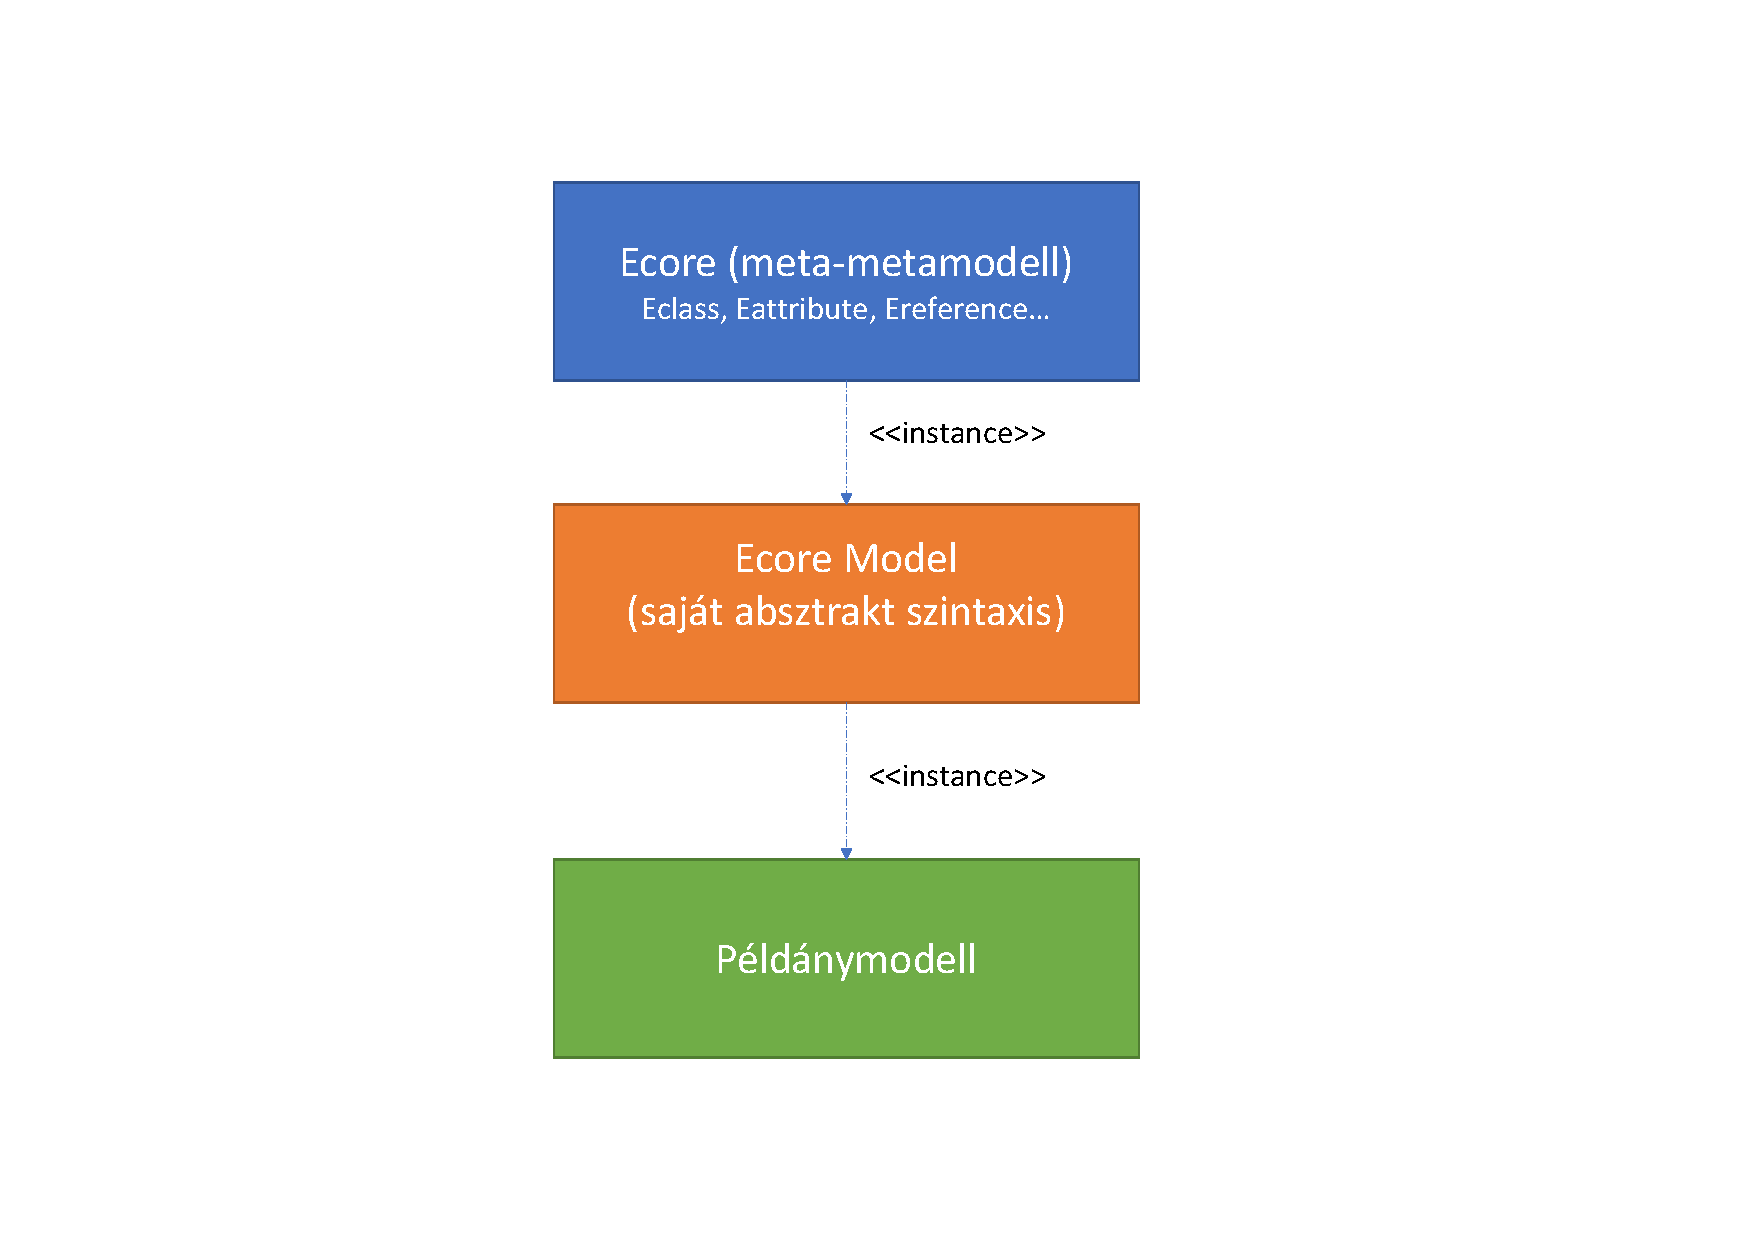
\includegraphics[width=100mm, keepaspectratio]{figures/ECore.pdf}
 	\caption{EMF meta szintek}
 	\label{fig:concept}
 \end{figure}
 

\section{Modell transzformációk}

Modellek származtatása más modellekből egy sokat alkalmazott megoldás a modell vezérelt fejlesztés során, hiszen így nem szükséges minden szakterület specifikus modellhez külön eszköz, ami ezekkel képes dolgozni. Ahhoz, ténylegesen származtatni tudjunk egy modellből egy másikat meg kell vizsgálni a szemantikájuk közötti kapcsolatokat és át kell hidalni a különbséget. Az ilyen jellegű szemantikai levezetést denotációs szemantikának nevezzük.

\begin{figure}[!ht]
	\centering
	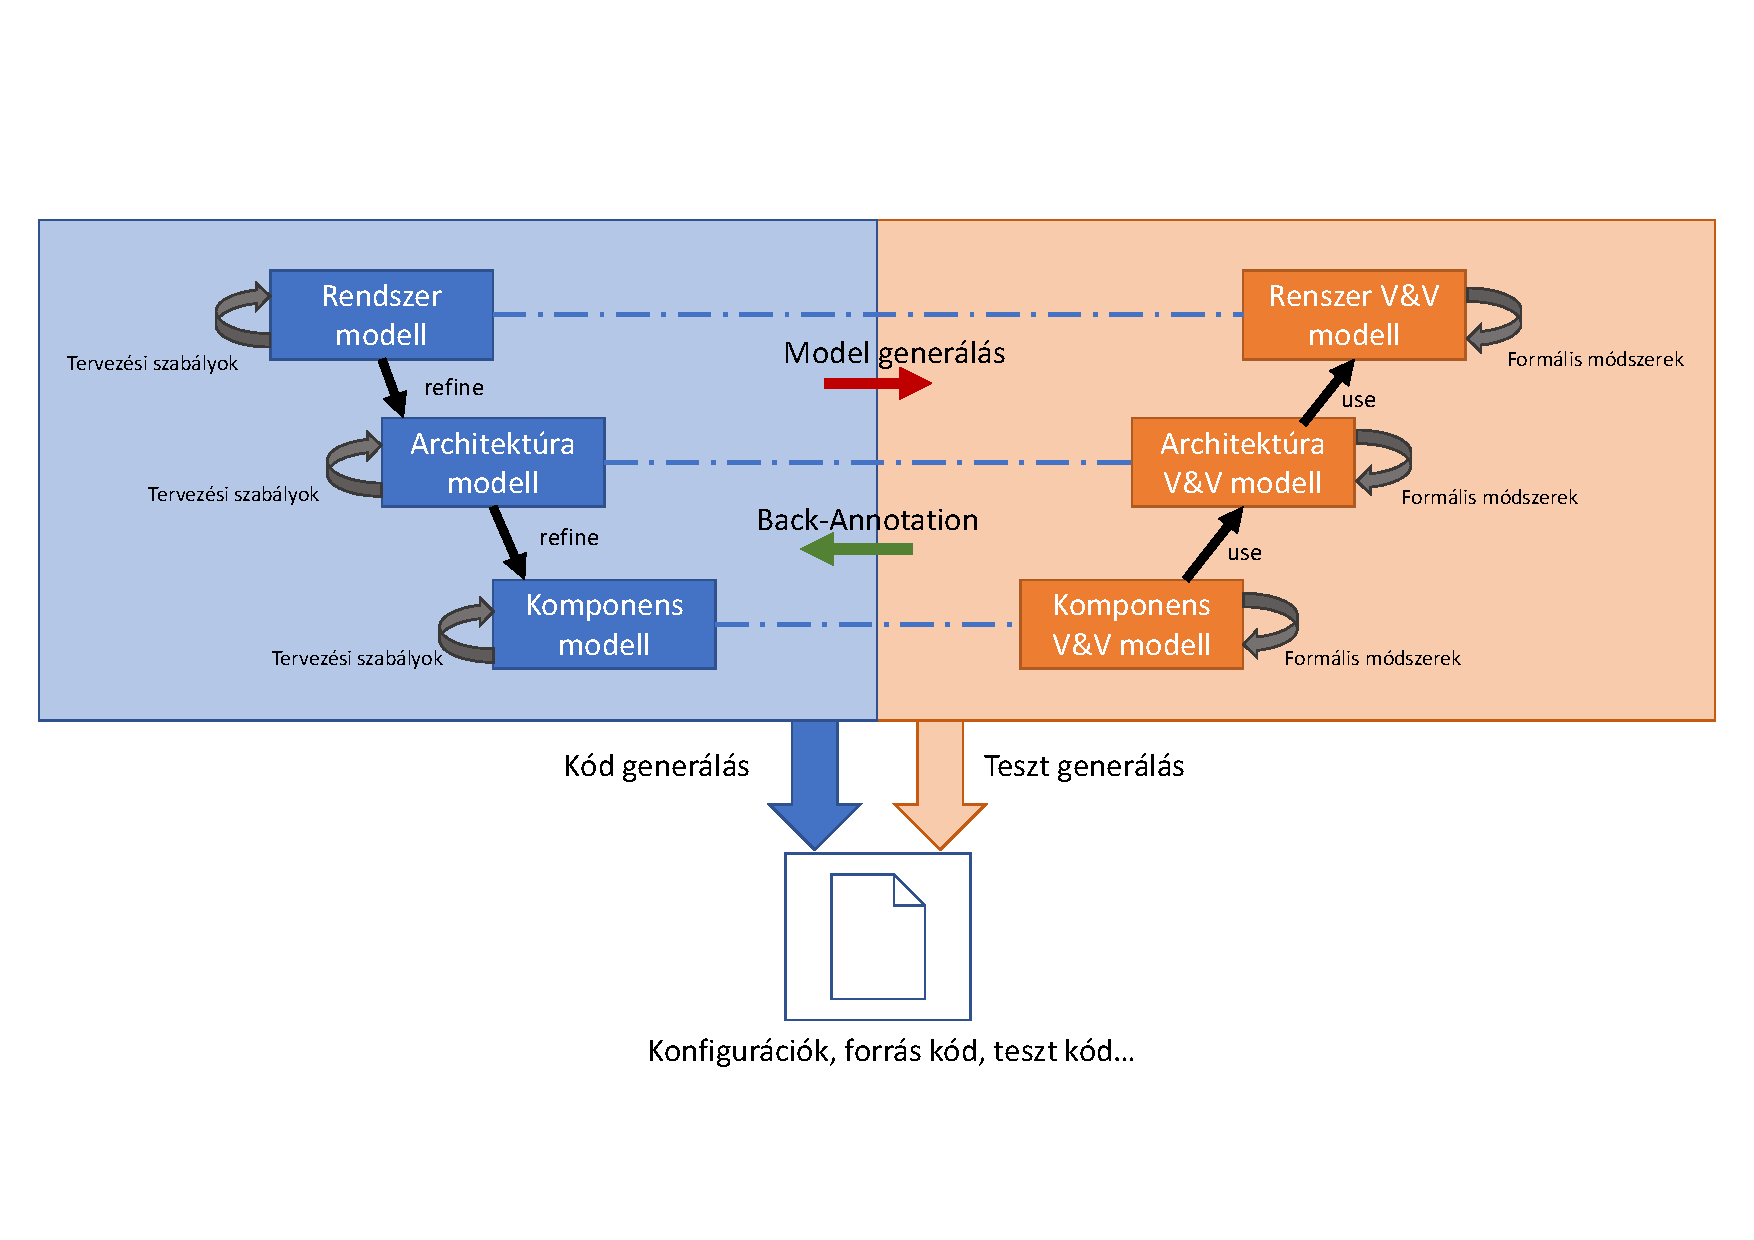
\includegraphics[width=100mm, keepaspectratio]{figures/Vmodel.pdf}
	\caption{Modell transzformációk alkalmazása a modell vezérelt fejlesztés során}
	\label{fig:concept}
\end{figure}

Modellek transzformálását sokféleképp végre lehet hajtani. Talán a legtriviálisabb megoldás a modell bejárása valamilyen általános célú programnyelv segítségével és a modell elemeinek egyenkénti feldolgozása. Ez a megoldás egyes esetekben elégséges lehet azonban nagyon nehéz karban tartani. Sokkal jobb megközelítés, hogy valamilyen lekérdező nyelvet alkalmazunk a modell bejárására. Ezek használata a programozó szemszögéből sokkal egyszerűbbek, hiszen deklaratív módon tudjuk megadni a lekérdezés specifikációját, ráadásul a lekérdezéseket különböző lekérdező motorok sokszor ki is optimalizálják, így egyes esetekben még hatékonyabb is lehet mint egy általános programozási nyelvvel történő keresések.

A VIATRA egy olyan technológia amivel modell lekérdezéseket és transzformációkat definiálhatunk. A lekérdezéseket egy speciális nyelv a Viatra Query Language (VQL) segítségével lehet leírni. Ez egy deklaratív nyelv amivel le tudjuk írni, hogy egyes elemek között milyen kapcsolatokat várunk.

\begin{lstlisting}[language=bash,frame=single,float=!ht]
pattern TranisitonsInStateMachine(stateMachine: StateMachine, transition: Transition){
	find RegionsInStatemachine(stateMachine, region);
	Region.transition(region, transition);
}
\end{lstlisting}

A VIATRA-val történő transzformációk két részből állnak: egy VQL nyelven leírt lekérdezés és egy imperatív módon leírt akció, ami minden illeszkedésre végrehajtódik.

\begin{lstlisting}[language=bash,frame=single,float=!ht]
	val transitionRule = createRule(transitionsInStateMachine).action[match | 
		//...
	].build
	
	//...
	
	def execute(){
		transitionRule.fireAllCurrent
	}
\end{lstlisting}

VIATRA-val kétféle transzformáció hozható létre. Batch transformation ami a programozó hívására elvégzi a transzformációt. Újbóli meghívás esetén a transzformációk ismét előröl végrehajtódnak. Illetve live transformation, ami figyeli a modellben történő változásokat (elemek törlése, létrehozása, frissítése) és ezeknek megfelelően hajt végre akciókat. Ennek során nem szükséges az egész modell leképzése, elég csak a változást érintő részek kezelése.


\section{MagicDraw pluginok}

A MagicDraw funkcionalításának bővítése pluginokkal lehetséges, ehhez a MagicDraw egy API-t biztosít melyet Open Api-nak neveznek ez lehetővé teszi, hogy hozzáférjünk a MagicDraw fő funkcióihoz. A plugin működéséhez két leíró fájlt kell előállítani. Az egyik a pluginDescriptor.xml ami a plugin telepítéséről és egyéb tulajdonságairól (vendor, név, verzió) tartalmaz információkat. Ez nem feltétlen szükséges a plugin futtatásához. A másik a plugin.xml ami nélkül a plugin nem fog betöltődni. Ez definiálja a plugin belépési pontját és a plugin classloaderjét. Az osztályok betöltéséhez a MagicDraw alapértelmezetten egy közös classpath-t használ, amin minden plugin osztozik. Ezt a plugin.xml-ben módosítani lehet, ha valamiért külön classloaderre lenne szükségünk a pluginunkhoz.

\paragraph{Példa:} plugin.xml tartalma
\begin{lstlisting}[language=bash,frame=single,float=!ht]
<plugin
id="magicdraw2gamma"
name="MagicDraw2Gamma Plugin"
internalVersion="1549381332"
version="1.0.0"
provider-name="BME-FTSRG"
class-lookup="LocalFirst"
ownClassloader="true"
class="hu.bme.mit.magicdraw2gamma.plugin.MagicDraw2GammaPlugin">

<requires>
	<required-plugin id="com.incquerylabs.v4md" name="V4MD" version="2.0.1" internalVersion="200003"/>
</requires>
<runtime></runtime>
</plugin>
\end{lstlisting}


A plugin.xml-ben hivatkozott osztálynak le kell öröklődnie a MagicDraw Plugin osztályából. A MagicDraw induláskor bejárja a plugins könyvtárát és beolvassa a plugin.xml-eket majd példányosítja és elindítja a ezeket, (meghívja az initet).

\begin{lstlisting}[language=bash,frame=single, float=t]

public class MyPlugin extends Plugin {

	@Override
	public void init() {
		//plugin started
	}

}
\end{lstlisting}

Az init során van lehetőségünk saját UI elemeink, működésünk hozzáadására a MagicDraw-hoz.

MagicDrawban ahhoz, hogy a modell elemekhez hozzáférjünk egy Session-t kell nyitni, ehhez a Sessionk manager osztály használható.

\begin{lstlisting}
	SessionManager.getInstance().startSession()
	...
\end{lstlisting}


\subsection{VIATRA használata MagicDrawban}

VIATRA használatára a MagicDrawban is lehetőségünk van. Ehhez egy open source plugint a V4MD-t érdemes használnunk. A plugin minden projekt megnyitásakor készít egy motort amivel lekérdezéseket és transzformációkat tudunk regisztrálni.

A motort a ViatraQueryAdapter osztály segítségével tudjuk elkérni vagy ha még nem létezett létrehozni.

\begin{lstlisting}
	ViatraQueryAdapter.getOrCreateEngine(project)
\end{lstlisting}


